\documentclass[a4paper,10pt]{article}
\usepackage[utf8]{inputenc}

% ----  Useful packages % ---- 
\usepackage{amsmath}
\usepackage{graphicx}
\usepackage{amsfonts}
\usepackage{amsthm}
\usepackage{amssymb}
\usepackage{makecell}
\usepackage{array}
\usepackage{booktabs}
\usepackage{multirow}
% ----  Useful packages % ---- 

\usepackage{wrapfig}
\usepackage{caption}
\usepackage{subcaption}
\usepackage{hyperref}
\hypersetup{
    colorlinks,
    citecolor=black,
    filecolor=black,
    linkcolor=black,
    urlcolor=black
}

\graphicspath{ {./images/} }

% ---- Set page size and margins replace ------
\usepackage[letterpaper,top=2cm,bottom=2cm,left=3cm,right=3cm,marginparwidth=1.75cm]{geometry}
% ---- Set page size and margins replace ------

% ------- NOTA ------
\theoremstyle{remark}
\newtheorem{note}{Note}[subsubsection]
% ------- NOTA ------

% ------- OSSERVAZIONE ------
\theoremstyle{definition}
\newtheorem{observation}{Osservazione}[subsection]
% ------- OSSERVAZIONE ------

% ------- DEFINIZIONE ------
\theoremstyle{plain}
\newtheorem{definition}{Definizione}[subsection]
% ------- DEFINIZIONE ------

% ------- ESEMPIO ------
\theoremstyle{definition}
\newtheorem{example}{Esempio}[subsection]
% ------- ESEMPIO ------

% ------- DIMOSTRAZIONE ------
\theoremstyle{definition}
\newtheorem{demostration}{Dimostrazione}[subsection]
% ------- DIMOSTRAZIONE ------

% ------- TEOREMA ------
\theoremstyle{definition}
\newtheorem{theorem}{Teorema}[subsection]
% ------- TEOREMA ------

% ------- COROLLARIO ------
\theoremstyle{plain}
\newtheorem{corollaries}{Corollario}[theorem]
% ------- COROLLARIO ------

% ------- PROPOSIZIONE ------
\theoremstyle{plain}
\newtheorem{proposition}{Proposizione}[subsection]
% ------- PROPOSIZIONE ------

% ---- Footer and header ---- 
\usepackage{fancyhdr}
\pagestyle{fancy}
\fancyhf{}
\fancyhead[LE,RO]{A.A 2022-2023}
\fancyhead[RE,LO]{Architettura e Sistemi Operativi}
\fancyfoot[RE,LO]{\rightmark}
\fancyfoot[LE,RO]{\thepage}

\renewcommand{\headrulewidth}{.5pt}
\renewcommand{\footrulewidth}{.5pt}
% ---- Footer and header ---- 

% ----  Language setting ---- 
\usepackage[italian, english]{babel}
% ----  Language setting ---- 

\usepackage{listings}
\usepackage{color}

\definecolor{dkgreen}{rgb}{0,0.6,0}
\definecolor{gray}{rgb}{0.5,0.5,0.5}
\definecolor{mauve}{rgb}{0.58,0,0.82}

\lstset{frame=tb,
  language=C,
  aboveskip=3mm,
  belowskip=3mm,
  showstringspaces=false,
  columns=flexible,
  basicstyle={\small\ttfamily},
  numbers=none,
  numberstyle=\tiny\color{gray},
  keywordstyle=\color{blue},
  commentstyle=\color{dkgreen},
  stringstyle=\color{mauve},
  breaklines=true,
  breakatwhitespace=true,
  tabsize=3
}

\title{\textbf{Architettura e Sistemi Operativi}}
\author{Realizzato da: Giuntoni Matteo e Ghirardini Filippo}
\date{A.A. 2023-2024}

\begin{document}
\begin{titlepage} %crea l'enviroment
	\begin{figure}[t] %inserisce le figure
		\centering
\includegraphics[width=0.98\textwidth]{marchio_unipi_pant541.png}
	\end{figure}
	\vspace{20mm}
	
	\begin{Large}
		\begin{center}
			\textbf{Dipartimento di Informatica\\ Corso di Laurea Triennale in Informatica\\}
			\vspace{20mm}
			{\huge{\bf Basi di dati}}\\
			\vspace{5mm}
			{\LARGE{Green City}}\\
			{\large{14 Maggio 2025}}
		\end{center}
	\end{Large}
	
	
	\vspace{36mm}
	\centering{
	\begin{minipage}[t]{0.47\textwidth}
		\centering
		{\large{\bf Autori:}\\ \large{Filippo Ghirardini (654829)}}
	\end{minipage}}
	
\end{titlepage}

\tableofcontents
\newpage
\maketitle
\begin{center}
    \vspace{-20pt}
    \rule{11cm}{.1pt} 
\end{center}
\newpage
\input{microarchitettura}
\input{retilogichecombinatorie}
% !TeX spellcheck = it_IT
\newpage
\section{Progetto di reti logiche sequenziali}
Le reti logiche sequenziali, avendo una memoria, riassume gli ingressi precedenti in \textbf{stati} del sistema. Questi sono composti da un insieme di bit detto \textbf{variabili di stato}.

\subsection{Macchine a stati finiti}
Le reti sequenziali \textbf{sincrone} possono essere rappresentate tramite \textbf{Finite State Machine}. Una FSM ha $M$ ingressi, $N$ uscite e $k$ bit di stato con $2^k$ possibili stati diversi. Riceve un segnale di \textit{clock} e a volte di \textit{reset}. Si compone di:
\begin{itemize}
	\item Logica di \textbf{stato prossimo} $\sigma$, implementata da reti combinatorie
	\begin{equation*}
		S: \text{IN} \times S \to S
	\end{equation*}
	\item Logica di \textbf{uscita} $\omega$, implementata da reti combinatorie
	\item \textbf{Registro di stato}
\end{itemize}
Le suddividiamo in due tipi:
\begin{itemize}
	\item Macchine di \textbf{Moore}: le uscite dipendono esclusivamente dallo stato attuale della macchina
	\begin{equation*}
		\omega: S \to \text{OUT}
	\end{equation*}
	\item Macchine di \textbf{Mealy}: le uscite dipendono sia dallo stato che dagli ingressi attuali
	\begin{equation*}
		\omega: \text{IN} \times S \to \text{OUT}
	\end{equation*}
\end{itemize}

\subsection{Registri}
\subsubsection{Latch SR}
Il latch SR (set \& reset) permette di memorizzare un bit ed è implementato come segue:
\begin{center}
	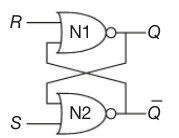
\includegraphics[scale=.4]{latchsr}
\end{center}
L'output non dipende solo dagli input ma anche dallo stato precedente, introducendo un ciclo.
\begin{observation}
	Nel caso in cui sia R che S valgono $1$, la rete non si stabilizza poiché non possiamo eseguire entrambe le operazioni di set e reset contemporaneamente.
\end{observation}

\subsubsection{Latch D}
Per risolvere la problematica del Latch SR, introduciamo un segnale di clock come segue:
\begin{center}
	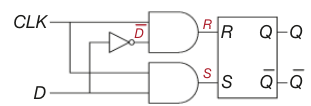
\includegraphics[scale=.4]{latchd}
\end{center}
In questo modo quando il clock vale zero (latch \textbf{opaco}), sia set che reset varranno zero, mentre se vale 1 (latch \textbf{trasparente}) set e reset avranno valori opposti in base all'operazione da fare.
\begin{observation}
	Dato che il clock ha un fronte di salita, il valore $D$ tenderà a stabilizzarsi solo dopo che il clock è alto, causando un ritardo.
\end{observation}

\subsubsection{Flip Flop D}
Per risolvere la problematica del ritardo nel Latch D, implementiamo il Flip Flop D utilizzando due Latch D: \textbf{slave} e \textbf{master}, rispettivamente con il clock non negato e negato.
\begin{center}
	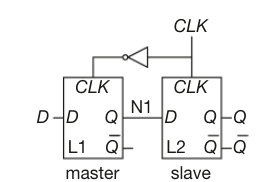
\includegraphics[scale=.4]{flipflopd}
\end{center}
Quando il clock vale $1$ lo slave è aperto alla scrittura e riceve eventuali aggiornamenti dal master per l'output da mostrare che sarà stato scritto su quest'ultimo nel ciclo precedente.\\
Quando il clock vale $0$ il master è aperto alla scrittura mentre lo slave no.\\
Questo permette che la stabilizzazione del clock avvenga solo nel master, rendendo più immediato l'output dallo slave.\\\\
È possibile implementare l'abilitazione alla scrittura tramite un bit \textbf{write enable} messo in AND con il bit del clock.

\subsubsection{Registro}
Il registro si implementa mettendo in parallelo $n$ Flip Flop D.

\subsection{Clock}
Nell'ambito delle prestazioni di reti sequenziali e combinatorie dobbiamo stimare la lunghezza del ciclo di clock, che dipende da:
\begin{itemize}
	\item Ritardi nelle porte logiche
	\item Complessità di $\sigma$
	\item Ritardi di propagazione e contaminazione dei registri
	\item $T_{\text{setup}}$: tempo minimo prima del fronte di salita del clock entro cui i valori degli ingressi devono essere cambiati e stabiliti
	\item $T_{\text{hold}}$: tempo in cui rimangono stabili gli ingressi dopo il fronte di salita del clock affinché il registro riesca a registrare il nuovo valore
	\begin{equation}
		T_{\text{hold}} \leq T_c^{\text{reg}} + T_c^\sigma
	\end{equation}
\end{itemize}

Otteniamo quindi che la stima minima della lunghezza del ciclo di clock è data da:
\begin{equation}
	\tau \geq T_p^{\text{reg}} + \max\{T_p^\omega, T_p^\sigma+T_{\text{setup}}\}
\end{equation}
% !TeX spellcheck = it_IT
\newpage
\section{Memorie}
Una memoria avrà:
\begin{itemize}
	\item Indirizzo da leggere, $k$ bit
	\item Indirizzo dove scrivere, $k$ bit
	\item Cosa scrivere, $n$ bit
	\item Write Enable, $1$ bit
	\item Valore letto, $n$ bit
\end{itemize}
\begin{center}
	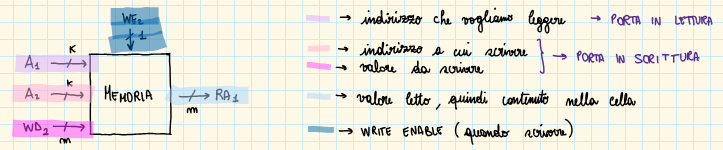
\includegraphics[scale=.6]{memoria}
\end{center}

\subsection{RAM}
Le memorie ad accesso casuale forniscono un tempo di accesso equivalente ad ogni cella.
\subsubsection{DRAM}
È una memoria \textbf{dinamica}, ovvero ha sempre bisogno di essere rinfrescata in quanto è composta da condensatori che mantengono la carica per un tempo limitato.\\
Quando eseguiamo una lettura il dato passa dal condensatore alla linea di bit e di conseguenza viene perso e ha bisogno di essere refreshato. Viceversa per quando scriviamo.
\begin{center}
	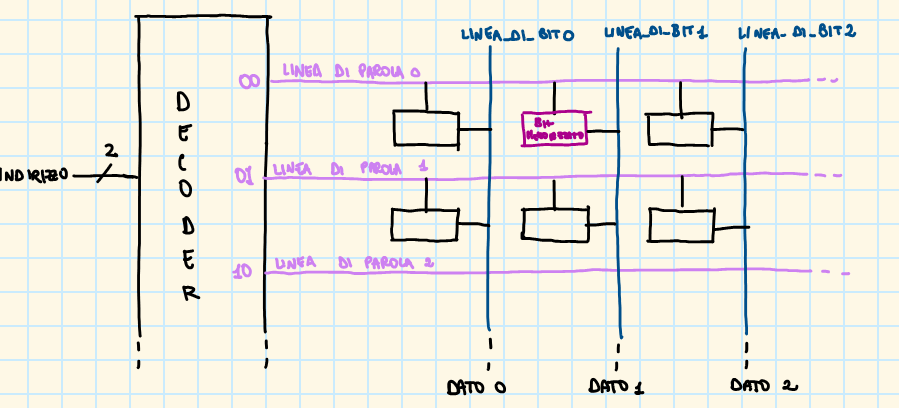
\includegraphics[scale=.3]{dram}
\end{center}

\subsubsection{SRAM}
A differenza delle DRAM utilizziamo più transistor ma questo ci permette di evitare l'operazione di refresh.
\begin{center}
	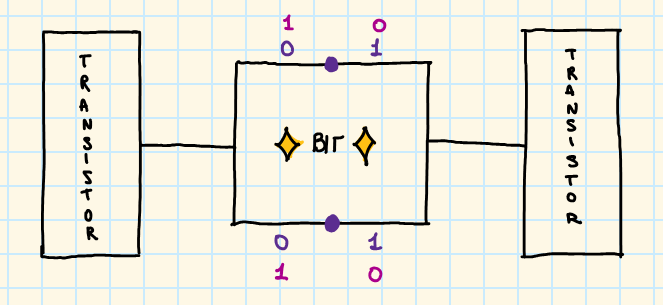
\includegraphics[scale=.3]{sram}
	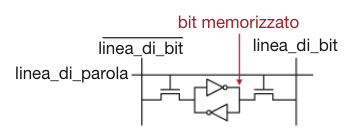
\includegraphics[scale=.4]{sram2}
\end{center}

\subsection{ROM e PROM}
La Read Only Memory è una memoria non volatile in sola lettura, strutturata in maniera molto simile alla DRAM e SRAM, con linee di parola, transistor e condensatori.\\
La \textbf{PROM} è una ROM programmabile, dove il programmatore può decidere i valori e poi salvarli bruciando i fusibili connessi alle celle di memoria.

\subsection{Memorie modulari}
Questo approccio alla progettazione di memoria prevede una mappatura in moduli più piccoli. La decomposizione può avvenire in due modi:
\begin{itemize}
	\item \textbf{Orizzontale}
	\begin{itemize}
		\item \textbf{Sequenziale}: date $n$ celle e $c$ moduli, dividiamo in $\frac{n}{c}$. Per cercare i dati usiamo poi i bit più significativi dato che i moduli posseggono un solo blocco
		\item \textbf{Interlacciata}: classifichiamo un bit si ed uno no, favorendo il parallelismo e diminuendo il costo di accesso
	\end{itemize}
	\item \textbf{Verticale}
\end{itemize}

\subsection{Memoria associativa}
In questo tipo di memoria associamo $k$ chiavi a $k$ locazioni nel momento in cui questa viene occupata da un valore. Nel momento in cui abbiamo una \textbf{hit} vuol dire che esiste quella chiave in memoria e possiamo cercarla.
\begin{center}
	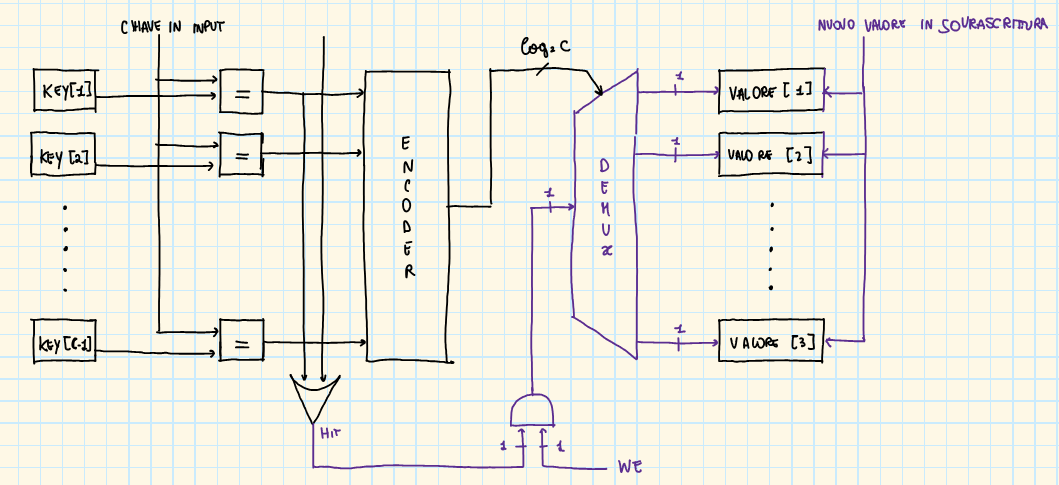
\includegraphics[scale=.4]{associativa}
\end{center}
\input{assembler}
\input{microarchitettura2}
\input{gerarchia-memoria}
\input{input-output.tex}
\input{disks.tex}
\input{cache}
\input{address_translation}
\input{kernel}
\input{concurrency}
\end{document}
